% -*-Latex-*-
%\documentclass[a4paper,landscape]{slides}
\documentclass[colorhighlight,coloremph]{beamer}
\usetheme{boxes}
\usepackage{color,soul}
\usepackage{graphicx}
%%\usepackage[pdftex]{graphicx}
\usepackage{asymptote}
\usepackage{amsmath}
%% packages for unicode
\usepackage{amssymb}
%% \usepackage{bbm}
%%\usepackage[greek,english]{babel}
\usepackage[english]{babel}

%% unicode translation
\usepackage{ucs}
\usepackage[utf8x]{inputenc}
%%\usepackage{autofe}
%%\usepackage{fancyvrb}

%% ODER: format ==         = "\mathrel{==}"
%% ODER: format /=         = "\neq "
%
%
\makeatletter
\@ifundefined{lhs2tex.lhs2tex.sty.read}%
  {\@namedef{lhs2tex.lhs2tex.sty.read}{}%
   \newcommand\SkipToFmtEnd{}%
   \newcommand\EndFmtInput{}%
   \long\def\SkipToFmtEnd#1\EndFmtInput{}%
  }\SkipToFmtEnd

\newcommand\ReadOnlyOnce[1]{\@ifundefined{#1}{\@namedef{#1}{}}\SkipToFmtEnd}
\usepackage{amstext}
\usepackage{amssymb}
\usepackage{stmaryrd}
\DeclareFontFamily{OT1}{cmtex}{}
\DeclareFontShape{OT1}{cmtex}{m}{n}
  {<5><6><7><8>cmtex8
   <9>cmtex9
   <10><10.95><12><14.4><17.28><20.74><24.88>cmtex10}{}
\DeclareFontShape{OT1}{cmtex}{m}{it}
  {<-> ssub * cmtt/m/it}{}
\newcommand{\texfamily}{\fontfamily{cmtex}\selectfont}
\DeclareFontShape{OT1}{cmtt}{bx}{n}
  {<5><6><7><8>cmtt8
   <9>cmbtt9
   <10><10.95><12><14.4><17.28><20.74><24.88>cmbtt10}{}
\DeclareFontShape{OT1}{cmtex}{bx}{n}
  {<-> ssub * cmtt/bx/n}{}
\newcommand{\tex}[1]{\text{\texfamily#1}}	% NEU

\newcommand{\Sp}{\hskip.33334em\relax}


\newcommand{\Conid}[1]{\mathit{#1}}
\newcommand{\Varid}[1]{\mathit{#1}}
\newcommand{\anonymous}{\kern0.06em \vbox{\hrule\@width.5em}}
\newcommand{\plus}{\mathbin{+\!\!\!+}}
\newcommand{\bind}{\mathbin{>\!\!\!>\mkern-6.7mu=}}
\newcommand{\rbind}{\mathbin{=\mkern-6.7mu<\!\!\!<}}% suggested by Neil Mitchell
\newcommand{\sequ}{\mathbin{>\!\!\!>}}
\renewcommand{\leq}{\leqslant}
\renewcommand{\geq}{\geqslant}
\usepackage{polytable}

%mathindent has to be defined
\@ifundefined{mathindent}%
  {\newdimen\mathindent\mathindent\leftmargini}%
  {}%

\def\resethooks{%
  \global\let\SaveRestoreHook\empty
  \global\let\ColumnHook\empty}
\newcommand*{\savecolumns}[1][default]%
  {\g@addto@macro\SaveRestoreHook{\savecolumns[#1]}}
\newcommand*{\restorecolumns}[1][default]%
  {\g@addto@macro\SaveRestoreHook{\restorecolumns[#1]}}
\newcommand*{\aligncolumn}[2]%
  {\g@addto@macro\ColumnHook{\column{#1}{#2}}}

\resethooks

\newcommand{\onelinecommentchars}{\quad-{}- }
\newcommand{\commentbeginchars}{\enskip\{-}
\newcommand{\commentendchars}{-\}\enskip}

\newcommand{\visiblecomments}{%
  \let\onelinecomment=\onelinecommentchars
  \let\commentbegin=\commentbeginchars
  \let\commentend=\commentendchars}

\newcommand{\invisiblecomments}{%
  \let\onelinecomment=\empty
  \let\commentbegin=\empty
  \let\commentend=\empty}

\visiblecomments

\newlength{\blanklineskip}
\setlength{\blanklineskip}{0.66084ex}

\newcommand{\hsindent}[1]{\quad}% default is fixed indentation
\let\hspre\empty
\let\hspost\empty
\newcommand{\NB}{\textbf{NB}}
\newcommand{\Todo}[1]{$\langle$\textbf{To do:}~#1$\rangle$}

\EndFmtInput
\makeatother
%
%
%
%
%
%
% This package provides two environments suitable to take the place
% of hscode, called "plainhscode" and "arrayhscode". 
%
% The plain environment surrounds each code block by vertical space,
% and it uses \abovedisplayskip and \belowdisplayskip to get spacing
% similar to formulas. Note that if these dimensions are changed,
% the spacing around displayed math formulas changes as well.
% All code is indented using \leftskip.
%
% Changed 19.08.2004 to reflect changes in colorcode. Should work with
% CodeGroup.sty.
%
\ReadOnlyOnce{polycode.fmt}%
\makeatletter

\newcommand{\hsnewpar}[1]%
  {{\parskip=0pt\parindent=0pt\par\vskip #1\noindent}}

% can be used, for instance, to redefine the code size, by setting the
% command to \small or something alike
\newcommand{\hscodestyle}{}

% The command \sethscode can be used to switch the code formatting
% behaviour by mapping the hscode environment in the subst directive
% to a new LaTeX environment.

\newcommand{\sethscode}[1]%
  {\expandafter\let\expandafter\hscode\csname #1\endcsname
   \expandafter\let\expandafter\endhscode\csname end#1\endcsname}

% "compatibility" mode restores the non-polycode.fmt layout.

\newenvironment{compathscode}%
  {\par\noindent
   \advance\leftskip\mathindent
   \hscodestyle
   \let\\=\@normalcr
   \let\hspre\(\let\hspost\)%
   \pboxed}%
  {\endpboxed\)%
   \par\noindent
   \ignorespacesafterend}

\newcommand{\compaths}{\sethscode{compathscode}}

% "plain" mode is the proposed default.
% It should now work with \centering.
% This required some changes. The old version
% is still available for reference as oldplainhscode.

\newenvironment{plainhscode}%
  {\hsnewpar\abovedisplayskip
   \advance\leftskip\mathindent
   \hscodestyle
   \let\hspre\(\let\hspost\)%
   \pboxed}%
  {\endpboxed%
   \hsnewpar\belowdisplayskip
   \ignorespacesafterend}

\newenvironment{oldplainhscode}%
  {\hsnewpar\abovedisplayskip
   \advance\leftskip\mathindent
   \hscodestyle
   \let\\=\@normalcr
   \(\pboxed}%
  {\endpboxed\)%
   \hsnewpar\belowdisplayskip
   \ignorespacesafterend}

% Here, we make plainhscode the default environment.

\newcommand{\plainhs}{\sethscode{plainhscode}}
\newcommand{\oldplainhs}{\sethscode{oldplainhscode}}
\plainhs

% The arrayhscode is like plain, but makes use of polytable's
% parray environment which disallows page breaks in code blocks.

\newenvironment{arrayhscode}%
  {\hsnewpar\abovedisplayskip
   \advance\leftskip\mathindent
   \hscodestyle
   \let\\=\@normalcr
   \(\parray}%
  {\endparray\)%
   \hsnewpar\belowdisplayskip
   \ignorespacesafterend}

\newcommand{\arrayhs}{\sethscode{arrayhscode}}

% The mathhscode environment also makes use of polytable's parray 
% environment. It is supposed to be used only inside math mode 
% (I used it to typeset the type rules in my thesis).

\newenvironment{mathhscode}%
  {\parray}{\endparray}

\newcommand{\mathhs}{\sethscode{mathhscode}}

% texths is similar to mathhs, but works in text mode.

\newenvironment{texthscode}%
  {\(\parray}{\endparray\)}

\newcommand{\texths}{\sethscode{texthscode}}

% The framed environment places code in a framed box.

\def\codeframewidth{\arrayrulewidth}
\RequirePackage{calc}

\newenvironment{framedhscode}%
  {\parskip=\abovedisplayskip\par\noindent
   \hscodestyle
   \arrayrulewidth=\codeframewidth
   \tabular{@{}|p{\linewidth-2\arraycolsep-2\arrayrulewidth-2pt}|@{}}%
   \hline\framedhslinecorrect\\{-1.5ex}%
   \let\endoflinesave=\\
   \let\\=\@normalcr
   \(\pboxed}%
  {\endpboxed\)%
   \framedhslinecorrect\endoflinesave{.5ex}\hline
   \endtabular
   \parskip=\belowdisplayskip\par\noindent
   \ignorespacesafterend}

\newcommand{\framedhslinecorrect}[2]%
  {#1[#2]}

\newcommand{\framedhs}{\sethscode{framedhscode}}

% The inlinehscode environment is an experimental environment
% that can be used to typeset displayed code inline.

\newenvironment{inlinehscode}%
  {\(\def\column##1##2{}%
   \let\>\undefined\let\<\undefined\let\\\undefined
   \newcommand\>[1][]{}\newcommand\<[1][]{}\newcommand\\[1][]{}%
   \def\fromto##1##2##3{##3}%
   \def\nextline{}}{\) }%

\newcommand{\inlinehs}{\sethscode{inlinehscode}}

% The joincode environment is a separate environment that
% can be used to surround and thereby connect multiple code
% blocks.

\newenvironment{joincode}%
  {\let\orighscode=\hscode
   \let\origendhscode=\endhscode
   \def\endhscode{\def\hscode{\endgroup\def\@currenvir{hscode}\\}\begingroup}
   %\let\SaveRestoreHook=\empty
   %\let\ColumnHook=\empty
   %\let\resethooks=\empty
   \orighscode\def\hscode{\endgroup\def\@currenvir{hscode}}}%
  {\origendhscode
   \global\let\hscode=\orighscode
   \global\let\endhscode=\origendhscode}%

\makeatother
\EndFmtInput
%

% the `doubleequals' macro is due to Jeremy Gibbons
\def\doubleequals{\mathrel{\unitlength 0.01em
  \begin{picture}(78,40)
    \put(7,34){\line(1,0){25}} \put(45,34){\line(1,0){25}}
    \put(7,14){\line(1,0){25}} \put(45,14){\line(1,0){25}}
  \end{picture}}}
%% If you remove the %format == command the lhs2TeX default yields ≡, which can be a problem


\newtheorem{thm}{Theorem}
\newtheorem{prop}{Proposition}
\newtheorem{dfn}{Definition}
\newtheorem{exm}{Example}
\newtheorem{cor}{Corollary}

\newcommand{\To}{\longrightarrow}
\newcommand{\Nat}{\mathbb{N}}
\newcommand{\Real}{\mathbb{R}}
\newcommand{\id}{\mathrm{id}}
\newcommand{\Hom}{\mathrm{Hom}}
\newcommand{\unit}{\mathrm{unit}}
\newcommand{\cat}[1]{\mathbf{#1}}

\def\commentbegin{\quad\{\ }
\def\commentend{\}}

\providecommand{\TODO}[1]{\textbf{TODO}\footnote{\textbf{#1}}}


\renewcommand{\hscodestyle}{%
   \setlength\leftskip{1em}%
   \small
}

%%\fvset{xleftmargin=0.0} %%\parindent}

\addheadbox{section}{
  \quad \tiny
  Formalizing reachability, viability and avoidability in the context of
  sequential decision problems
  \ $\rightarrow$ \
  \color{blue} \insertsection
}
%\addfootbox{section}{\quad \tiny Modelling Strategy Seminar, PIK, June
%  2012}
\title{Formalizing reachability, viability and avoidability in the
  context of sequential decision problems}

\author{Nicola Botta, Cezar Ionescu, Patrik Jansson}

\begin{document}
\date{}
\frame{\maketitle}

%% -------------------------------------------------------------------

\section{Outline}

%% -------------------------------------------------------------------

\begin{frame}[fragile]
\frametitle{Outline}
%
\begin{itemize}
\vspace{0.3\normalbaselineskip}
\item Why formalizing what?
\vspace{0.3\normalbaselineskip}
\item Minimal goals
\vspace{0.3\normalbaselineskip}
\item Sequential decision problems
\vspace{0.3\normalbaselineskip}
\item Reachability and viability
\vspace{0.3\normalbaselineskip}
\item Avoidability
\end{itemize}
\vfill
%
\end{frame}


%% -------------------------------------------------------------------

\section{Why formalizing what?}

%% -------------------------------------------------------------------

\begin{frame}[fragile]
\frametitle{Why formalizing what?}
%
\begin{itemize}
  \vspace{0.3\normalbaselineskip}
  \item<1-> \emph{International emissions trading: Good or bad?},
    Holtsmark \& Sommervoll, 2012: ``[\ldots] we find that an agreement
    with international emissions trading leads to \textcolor<2-3>{red}{increased emissions}
    and \textcolor<2-3>{red}{reduced efficiency}.''
  \vspace{0.3\normalbaselineskip}
  \item<1-> \emph{The case for international emission trade in the
    absence of cooperative climate policy}, Carbone et al., 2009:
    ``[\ldots] we find that emission trade agreements \textcolor<3>{green}{can be effective}
    [\ldots]''
  \vspace{0.3\normalbaselineskip}
  \item<4-> \emph{Confronting Climate Change: \textcolor{red}{Avoiding the Unmanageable
    and Managing the Unavoidable}}, P. Raven, R. Bierbaum, J. Holdren,
    UN-Sigma Xi Climate Change Report, 2007.
\end{itemize}
%
\end{frame}

%% -------------------------------------------------------------------

\begin{frame}[fragile]
\frametitle{Why formalizing what?}
%
Some notion of avoidability is implicit in the WG3\_IPCC\_AR5\_2014
definitions of
\begin{itemize}
  \vspace{0.3\normalbaselineskip}
  \item<1-> \emph{mitigation}: ``A human intervention to reduce the
    sources or enhance the sinks of greenhouse gases'' \onslide<2->{$\Rightarrow$
    \textcolor{red}{avoid high atmospheric GHG concentrations}}
  \vspace{0.3\normalbaselineskip}
  \item<3-> \emph{adaptation}: ``The process of adjustment to actual or
    expected climate and its effects \dots to moderate harm or exploit
    beneficial opportunities'' \onslide<4->{$\Rightarrow$ \textcolor{red}{avoid
      too much harm, realize beneficial opportunities}}
\end{itemize}
%
\vspace{0.3\normalbaselineskip} \onslide<5->{But what does it mean (for
  atmospheric GHG concentrations) to be \emph{avoidable}?}
%
\end{frame}

%% -------------------------------------------------------------------

\begin{frame}[fragile]
\frametitle{Why formalizing what?}
%
\begin{figure}[h]                                                                                                         
  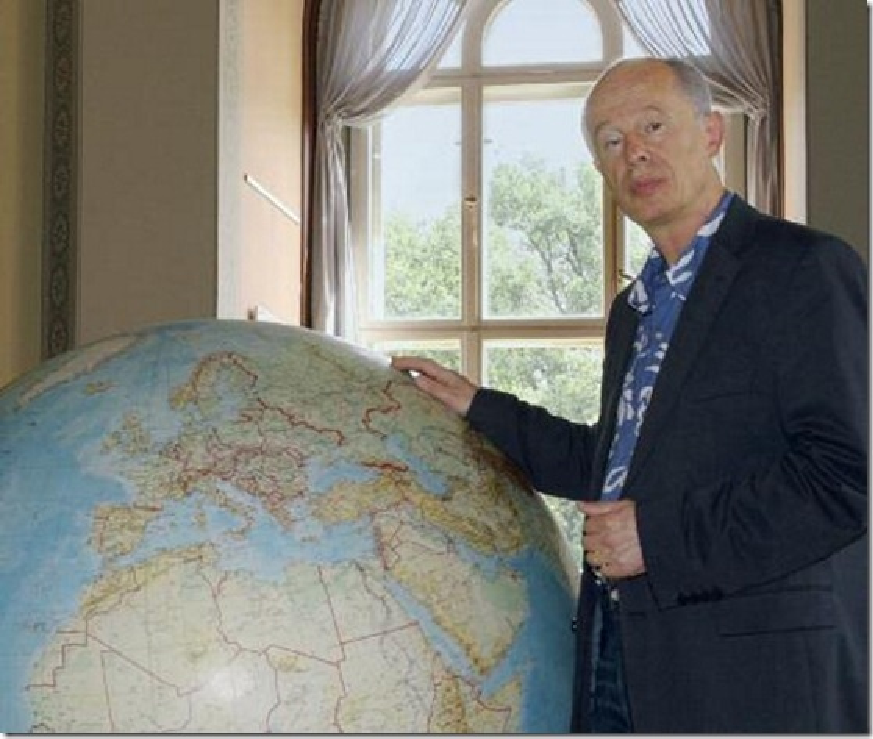
\includegraphics[scale=0.4]{schellnhuber.pdf}                                                                           
\end{figure}                                                                                                              
\begin{tabular}{p{0.9\textwidth}}                                                                                         
``Die Rolle der Klimaforschung bleibt weiterhin, die Problemfakten auf                                                    
den Tisch zu knallen und Optionen f\"ur geeignete L\"osungswege zu                                                        
identifizieren.'' \\                                                                                                      
\end{tabular}                                                                                                             
                                                                                                                          
\hfill H.-J. Schellnhuber in \emph{Frankfurter Allgemeine} from 2012-06-19 \\  
%
\end{frame}

%% -------------------------------------------------------------------

\begin{frame}[fragile]
\frametitle{Why formalizing what?}
%
But how can we produce ``hard facts'' if the notions used to phrase
specific, concrete problems are ambiguous, devoid of precise, well
established, meanings?
%
\end{frame}

%% -------------------------------------------------------------------

\section{Minimal goals}

%% -------------------------------------------------------------------

\begin{frame}[fragile]
\frametitle{Minimal goals}
%
\begin{itemize}
  \vspace{0.3\normalbaselineskip}
  \pause
  \item Explain what it means for future (possibly harmful) states to be
    avoidable [reachable, viable, \dots]
  \vspace{0.3\normalbaselineskip}
  \pause
  \item Explain under which conditions is it \emph{decidable}
    whether future states are avoidable [reachable, viable, \dots] or not
\end{itemize}
\pause
Further questions, goals
\begin{itemize}
  \vspace{0.3\normalbaselineskip}
  \pause
  \item Can one exploit decidability to derive useful avoidability
    (levity?) measures?
  \vspace{0.3\normalbaselineskip}
  \pause
  \item Can one refine decidable notions of viability, avoidability to
    derive operational notions (measures?) of sustainability,
    adaptability, resilience?
\end{itemize}
%
\end{frame}


%% -------------------------------------------------------------------

\section{Sequential decision problems}

%% -------------------------------------------------------------------

\begin{frame}[fragile]
\frametitle{Sequential decision problems (intuition)} % show only the states for n+1

\pause
\begin{figure}[h]
 \begin{asy}
  include graph;
  size(11cm);
  int o = 1;
  int l = 8;
  int h = 4;
  pair A, B, C, D;
  int x = 0;
  real[] midxs1;
  real[] midys1;
  real[] midxs2;
  real[] midys2;
  for (int i = 0; i < 6; ++i)
  {
    x = i * (l + o);
    midxs1.push(x + l/2);
    midys1.push(0);
    if (i == 3) 
    {
      real a = (l+2*o)/3;
      for (int j = 1; j < 4; ++j)
      {
        draw(Circle((x-2*o+j*a-0.5,2),.5), blue);
      }
    } else
    {
    A=(x,0); B=(x,h); C=(x+l,h); D=(x+l,0);
    draw(A--B--C--D--A,blue);
    }
  }
  int cx = l+o+floor(l/2);
  int cy = h + h + h;
  int cr = floor(h);
  draw(Circle((cx,cy),cr), white);
  draw(Circle((cx-1.5,cy-1.5),0.5), white);
  draw(Circle((cx+2,cy+2),0.5), white);
  draw(Circle((cx-0.2,cy+1.5),0.5), white);
  draw(Circle((cx+1.8,cy-1.2),0.5), white);
  draw(Circle((cx+1.8,cy-1.2),0.5), white);
  label("n+1 steps left", (x+17,2));
  int y = -15;
  for (int i = 0; i < 6; ++i)
  {
    x = i * (l + o);
    midxs2.push(x + l/2);
    midys2.push(y+h);
    if (i == 3) 
    {
      real a = (l+2*o)/3;
      for (int j = 1; j < 4; ++j)
      {
        draw(Circle((x-2*o+j*a-0.5,2+y),.5), white);
      }
    } else
    {
    A=(x,y); B=(x,y+h); C=(x+l,y+h); D=(x+l,y);
    if (i == 0 | i == 5)
    {
    draw(A--B--C--D--A,white);
    } else
    {
    draw(A--B--C--D--A,white);
    }
    }
  }
  label("n steps left", (x+17,y+2), white);
  for (int j = 5; j < 5; ++j)
  {
    draw((midxs1[1],midys1[1])--(midxs2[j],midys2[j]), white, EndArrow);
  }


\end{asy}
\end{figure}

\vfill

\end{frame}

%% -------------------------------------------------------------------

\begin{frame}[fragile]
\frametitle{You are here\ldots} % show only the states for
                                % n+1 and fill the state we're in

\begin{figure}[h]
 \begin{asy}
  include graph;
  size(11cm);
  int o = 1;
  int l = 8;
  int h = 4;
  pair A, B, C, D;
  int x = 0;
  real[] midxs1;
  real[] midys1;
  real[] midxs2;
  real[] midys2;
  for (int i = 0; i < 6; ++i)
  {
    x = i * (l + o);
    midxs1.push(x + l/2);
    midys1.push(0);
    if (i == 3) 
    {
      real a = (l+2*o)/3;
      for (int j = 1; j < 4; ++j)
      {
        draw(Circle((x-2*o+j*a-0.5,2),.5), blue);
      }
    } else
    {
      A=(x,0); B=(x,h); C=(x+l,h); D=(x+l,0);
      if (i == 1) {
         fill(A--B--C--D--cycle,blue);
      } else {
         draw(A--B--C--D--A,blue);
      }
    }
  }
  int cx = l+o+floor(l/2);
  int cy = h + h + h;
  int cr = floor(h);
  draw(Circle((cx,cy),cr), white);
  draw(Circle((cx-1.5,cy-1.5),0.5), white);
  draw(Circle((cx+2,cy+2),0.5), white);
  draw(Circle((cx-0.2,cy+1.5),0.5), white);
  draw(Circle((cx+1.8,cy-1.2),0.5), white);
  draw(Circle((cx+1.8,cy-1.2),0.5), white);
  label("n+1 steps left", (x+17,2));
  int y = -15;
  for (int i = 0; i < 6; ++i)
  {
    x = i * (l + o);
    midxs2.push(x + l/2);
    midys2.push(y+h);
    if (i == 3) 
    {
      real a = (l+2*o)/3;
      for (int j = 1; j < 4; ++j)
      {
        draw(Circle((x-2*o+j*a-0.5,2+y),.5), white);
      }
    } else
    {
    A=(x,y); B=(x,y+h); C=(x+l,y+h); D=(x+l,y);
    if (i == 0 | i == 5)
    {
    draw(A--B--C--D--A,white);
    } else
    {
    draw(A--B--C--D--A,white);
    }
    }
  }
  label("n steps left", (x+17,y+2), white);
  for (int j = 5; j < 5; ++j)
  {
    draw((midxs1[1],midys1[1])--(midxs2[j],midys2[j]), white, EndArrow);
  }


\end{asy}
\end{figure}

\vfill

\end{frame}

%% -------------------------------------------------------------------

\begin{frame}[fragile]
\frametitle{These are your options\ldots} % show only the states for
                                % n+1 and fill the state we're in and
                                % show the available controls

\begin{figure}[h]
 \begin{asy}
  include graph;
  size(11cm);
  int o = 1;
  int l = 8;
  int h = 4;
  pair A, B, C, D;
  int x = 0;
  real[] midxs1;
  real[] midys1;
  real[] midxs2;
  real[] midys2;
  for (int i = 0; i < 6; ++i)
  {
    x = i * (l + o);
    midxs1.push(x + l/2);
    midys1.push(0);
    if (i == 3) 
    {
      real a = (l+2*o)/3;
      for (int j = 1; j < 4; ++j)
      {
        draw(Circle((x-2*o+j*a-0.5,2),.5), blue);
      }
    } else
    {
      A=(x,0); B=(x,h); C=(x+l,h); D=(x+l,0);
      if (i == 1) {
         fill(A--B--C--D--cycle,blue);
      } else {
         draw(A--B--C--D--A,blue);
      }
    }
  }
  int cx = l+o+floor(l/2);
  int cy = h + h + h;
  int cr = floor(h);
  draw(Circle((cx,cy),cr), blue);
  draw(Circle((cx-1.5,cy-1.5),0.5), green);
  draw(Circle((cx+2,cy+2),0.5), yellow);
  draw(Circle((cx-0.2,cy+1.5),0.5), brown);
  draw(Circle((cx+1.8,cy-1.2),0.5), red);
  draw(Circle((cx-2.1,cy+1.2),0.5), black);
  label("n+1 steps left", (x+17,2));
  int y = -15;
  for (int i = 0; i < 6; ++i)
  {
    x = i * (l + o);
    midxs2.push(x + l/2);
    midys2.push(y+h);
    if (i == 3) 
    {
      real a = (l+2*o)/3;
      for (int j = 1; j < 4; ++j)
      {
        draw(Circle((x-2*o+j*a-0.5,2+y),.5), white);
      }
    } else
    {
    A=(x,y); B=(x,y+h); C=(x+l,y+h); D=(x+l,y);
    if (i == 0 | i == 5)
    {
    draw(A--B--C--D--A,white);
    } else
    {
    draw(A--B--C--D--A,white);
    }
    }
  }
  label("n steps left", (x+17,y+2), white);
  for (int j = 5; j < 5; ++j)
  {
    draw((midxs1[1],midys1[1])--(midxs2[j],midys2[j]), white, EndArrow);
  }


\end{asy}
\end{figure}

\vfill

\end{frame}

%% -------------------------------------------------------------------

\begin{frame}[fragile]
\frametitle{Pick one!} % show only the states for
                                % n+1 and fill the state we're in
                                % show the available controls and fill
                                % in a choice

\begin{figure}[h]
 \begin{asy}
  include graph;
  size(11cm);
  int o = 1;
  int l = 8;
  int h = 4;
  pair A, B, C, D;
  int x = 0;
  real[] midxs1;
  real[] midys1;
  real[] midxs2;
  real[] midys2;
  for (int i = 0; i < 6; ++i)
  {
    x = i * (l + o);
    midxs1.push(x + l/2);
    midys1.push(0);
    if (i == 3) 
    {
      real a = (l+2*o)/3;
      for (int j = 1; j < 4; ++j)
      {
        draw(Circle((x-2*o+j*a-0.5,2),.5), blue);
      }
    } else
    {
      A=(x,0); B=(x,h); C=(x+l,h); D=(x+l,0);
      if (i == 1) {
         fill(A--B--C--D--cycle,blue);
      } else {
         draw(A--B--C--D--A,blue);
      }
    }
  }
  int cx = l+o+floor(l/2);
  int cy = h + h + h;
  int cr = floor(h);
  draw(Circle((cx,cy),cr), blue);
  fill(Circle((cx-1.5,cy-1.5),0.5), green);
  draw(Circle((cx+2,cy+2),0.5), yellow);
  draw(Circle((cx-0.2,cy+1.5),0.5), brown);
  draw(Circle((cx+1.8,cy-1.2),0.5), red);
  draw(Circle((cx-2.1,cy+1.2),0.5), black);
  label("n+1 steps left", (x+17,2));
  int y = -15;
  for (int i = 0; i < 6; ++i)
  {
    x = i * (l + o);
    midxs2.push(x + l/2);
    midys2.push(y+h);
    if (i == 3) 
    {
      real a = (l+2*o)/3;
      for (int j = 1; j < 4; ++j)
      {
        draw(Circle((x-2*o+j*a-0.5,2+y),.5), white);
      }
    } else
    {
    A=(x,y); B=(x,y+h); C=(x+l,y+h); D=(x+l,y);
    if (i == 0 | i == 5)
    {
    draw(A--B--C--D--A,white);
    } else
    {
    draw(A--B--C--D--A,white);
    }
    }
  }
  label("n steps left", (x+17,y+2), white);
  for (int j = 5; j < 5; ++j)
  {
    draw((midxs1[1],midys1[1])--(midxs2[j],midys2[j]), white, EndArrow);
  }


\end{asy}
\end{figure}

\vfill

\end{frame}

%% -------------------------------------------------------------------

\begin{frame}[fragile]
\frametitle{Advance one step\ldots} % transition from n+1 to n

\begin{figure}[h]
 \begin{asy}
  include graph;
  size(11cm);
  int o = 1;
  int l = 8;
  int h = 4;
  pair A, B, C, D;
  int x = 0;
  real[] midxs1;
  real[] midys1;
  real[] midxs2;
  real[] midys2;
  for (int i = 0; i < 6; ++i)
  {
    x = i * (l + o);
    midxs1.push(x + l/2);
    midys1.push(0);
    if (i == 3) 
    {
      real a = (l+2*o)/3;
      for (int j = 1; j < 4; ++j)
      {
        draw(Circle((x-2*o+j*a-0.5,2),.5), blue);
      }
    } else
    {
      A=(x,0); B=(x,h); C=(x+l,h); D=(x+l,0);
      if (i == 1) {
         fill(A--B--C--D--cycle,blue);
      } else {
         draw(A--B--C--D--A,blue);
      }
    }
  }
  int cx = l+o+floor(l/2);
  int cy = h + h + h;
  int cr = floor(h);
  draw(Circle((cx,cy),cr), blue);
  fill(Circle((cx-1.5,cy-1.5),0.5), green);
  draw(Circle((cx+2,cy+2),0.5), yellow);
  draw(Circle((cx-0.2,cy+1.5),0.5), brown);
  draw(Circle((cx+1.8,cy-1.2),0.5), red);
  draw(Circle((cx-2.1,cy+1.2),0.5), black);
  label("n+1 steps left", (x+17,2));
  int y = -15;
  for (int i = 0; i < 6; ++i)
  {
    x = i * (l + o);
    midxs2.push(x + l/2);
    midys2.push(y+h);
    if (i == 3) 
    {
      real a = (l+2*o)/3;
      for (int j = 1; j < 4; ++j)
      {
        draw(Circle((x-2*o+j*a-0.5,2+y),.5), blue);
      }
    } else
    {
    A=(x,y); B=(x,y+h); C=(x+l,y+h); D=(x+l,y);
    if (i == 0 | i == 5)
    {
    draw(A--B--C--D--A,white);
    } else
    {
    draw(A--B--C--D--A,blue);
    }
    }
  }
  label("n steps left", (x+17,y+2), black);
  for (int j = 2; j < 3; ++j)
  {
    draw((midxs1[1],midys1[1])--(midxs2[j],midys2[j]), black,
    EndArrow);
  }


\end{asy}
\end{figure}

\vfill

\end{frame}

%% -------------------------------------------------------------------

\begin{frame}[fragile]
\frametitle{\ldots collect rewards \ldots} % we are now in n and we
                                           % collect our reward

\begin{figure}[h]
 \begin{asy}
  include graph;
  size(11cm);
  int o = 1;
  int l = 8;
  int h = 4;
  pair A, B, C, D;
  int x = 0;
  real[] midxs1;
  real[] midys1;
  real[] midxs2;
  real[] midys2;
  for (int i = 0; i < 6; ++i)
  {
    x = i * (l + o);
    midxs1.push(x + l/2);
    midys1.push(0);
    if (i == 3) 
    {
      real a = (l+2*o)/3;
      for (int j = 1; j < 4; ++j)
      {
        draw(Circle((x-2*o+j*a-0.5,2),.5), blue);
      }
    } else
    {
      A=(x,0); B=(x,h); C=(x+l,h); D=(x+l,0);
      if (i == 1) {
         draw(A--B--C--D--A,blue);
      } else {
         draw(A--B--C--D--A,blue);
      }
    }
  }
  int cx = l+o+floor(l/2);
  int cy = h + h + h;
  int cr = floor(h);
  draw(Circle((cx,cy),cr), blue);
  fill(Circle((cx-1.5,cy-1.5),0.5), green);
  draw(Circle((cx+2,cy+2),0.5), yellow);
  draw(Circle((cx-0.2,cy+1.5),0.5), brown);
  draw(Circle((cx+1.8,cy-1.2),0.5), red);
  draw(Circle((cx-2.1,cy+1.2),0.5), black);
  label("n+1 steps left", (x+17,2));
  int y = -15;
  for (int i = 0; i < 6; ++i)
  {
    x = i * (l + o);
    midxs2.push(x + l/2);
    midys2.push(y+h);
    if (i == 3) 
    {
      real a = (l+2*o)/3;
      for (int j = 1; j < 4; ++j)
      {
        draw(Circle((x-2*o+j*a-0.5,2+y),.5), blue);
      }
    } else
    {
    A=(x,y); B=(x,y+h); C=(x+l,y+h); D=(x+l,y);
    if (i == 0 | i == 5)
    {
    draw(A--B--C--D--A,white);
    } else
    {
      if (i == 2) {
         fill (A--B--C--D--cycle,blue);
      } else {
         draw(A--B--C--D--A,blue);
      }
    }
    }
  }
  label("n steps left", (x+17,y+2), black);
  for (int j = 2; j < 3; ++j)
  {
    draw((midxs1[1],midys1[1])--(midxs2[j],midys2[j]), black,
    EndArrow);
  }


\end{asy}
\end{figure}

\vfill

\end{frame}

%% -------------------------------------------------------------------

\begin{frame}[fragile]
\frametitle{\ldots and go!} % only states at n steps left


\begin{figure}[h]
 \begin{asy}
  include graph;
  size(11cm);
  int o = 1;
  int l = 8;
  int h = 4;
  pair A, B, C, D;
  int x = 0;
  real[] midxs1;
  real[] midys1;
  real[] midxs2;
  real[] midys2;
  for (int i = 0; i < 6; ++i)
  {
    x = i * (l + o);
    midxs1.push(x + l/2);
    midys1.push(0);
    if (i == 3) 
    {
      real a = (l+2*o)/3;
      for (int j = 1; j < 4; ++j)
      {
        draw(Circle((x-2*o+j*a-0.5,2),.5), white);
      }
    } else
    {
      A=(x,0); B=(x,h); C=(x+l,h); D=(x+l,0);
      if (i == 1) {
         draw(A--B--C--D--A,white);
      } else {
         draw(A--B--C--D--A,white);
      }
    }
  }
  int cx = l+o+floor(l/2);
  int cy = h + h + h;
  int cr = floor(h);
  draw(Circle((cx,cy),cr), white);
  fill(Circle((cx-1.5,cy-1.5),0.5), white);
  draw(Circle((cx+2,cy+2),0.5), white);
  draw(Circle((cx-0.2,cy+1.5),0.5), white);
  draw(Circle((cx+1.8,cy-1.2),0.5), white);
  draw(Circle((cx-2.1,cy+1.2),0.5), white);
  label("n+1 steps left", (x+17,2), white);
  int y = -15;
  for (int i = 0; i < 6; ++i)
  {
    x = i * (l + o);
    midxs2.push(x + l/2);
    midys2.push(y+h);
    if (i == 3) 
    {
      real a = (l+2*o)/3;
      for (int j = 1; j < 4; ++j)
      {
        draw(Circle((x-2*o+j*a-0.5,2+y),.5), blue);
      }
    } else
    {
    A=(x,y); B=(x,y+h); C=(x+l,y+h); D=(x+l,y);
    if (i == 0 | i == 5)
    {
    draw(A--B--C--D--A,white);
    } else
    {
      if (i == 2) {
         fill (A--B--C--D--cycle,blue);
      } else {
         draw(A--B--C--D--A,blue);
      }
    }
    }
  }
  label("n steps left", (x+17,y+2), black);
  for (int j = 2; j < 3; ++j)
  {
    draw((midxs1[1],midys1[1])--(midxs2[j],midys2[j]), white,
    EndArrow);
  }


\end{asy}
\end{figure}

\vfill

\end{frame}

%% -------------------------------------------------------------------

\begin{frame}[fragile]
\frametitle{General sequential decision problems (intuition)} % non-deterministic transition

\pause
\begin{figure}[h]
 \begin{asy}
  include graph;
  size(11cm);
  int o = 1;
  int l = 8;
  int h = 4;
  pair A, B, C, D;
  int x = 0;
  real[] midxs1;
  real[] midys1;
  real[] midxs2;
  real[] midys2;
  for (int i = 0; i < 6; ++i)
  {
    x = i * (l + o);
    midxs1.push(x + l/2);
    midys1.push(0);
    if (i == 3) 
    {
      real a = (l+2*o)/3;
      for (int j = 1; j < 4; ++j)
      {
        draw(Circle((x-2*o+j*a-0.5,2),.5), blue);
      }
    } else
    {
      A=(x,0); B=(x,h); C=(x+l,h); D=(x+l,0);
      if (i == 1) {
         fill(A--B--C--D--cycle,blue);
      } else {
         draw(A--B--C--D--A,blue);
      }
    }
  }
  int cx = l+o+floor(l/2);
  int cy = h + h + h;
  int cr = floor(h);
  draw(Circle((cx,cy),cr), blue);
  fill(Circle((cx-1.5,cy-1.5),0.5), green);
  draw(Circle((cx+2,cy+2),0.5), yellow);
  draw(Circle((cx-0.2,cy+1.5),0.5), brown);
  draw(Circle((cx+1.8,cy-1.2),0.5), red);
  draw(Circle((cx-2.1,cy+1.2),0.5), black);
  label("n+1 steps left", (x+17,2));
  int y = -15;
  for (int i = 0; i < 6; ++i)
  {
    x = i * (l + o);
    midxs2.push(x + l/2);
    midys2.push(y+h);
    if (i == 3) 
    {
      real a = (l+2*o)/3;
      for (int j = 1; j < 4; ++j)
      {
        draw(Circle((x-2*o+j*a-0.5,2+y),.5), blue);
      }
    } else
    {
    A=(x,y); B=(x,y+h); C=(x+l,y+h); D=(x+l,y);
    if (i == 0 | i == 5)
    {
    draw(A--B--C--D--A,white);
    } else
    {
    draw(A--B--C--D--A,blue);
    }
    }
  }
  label("n steps left", (x+17,y+2), black);
  for (int j = 1; j < 5; ++j)
  {
    draw((midxs1[1],midys1[1])--(midxs2[j],midys2[j]), red,
    EndArrow);
  }


\end{asy}
\end{figure}

\vfill

\end{frame}

%% -------------------------------------------------------------------

\begin{frame}[fragile]
\frametitle{Sequential decision problems (notation)}

\begin{figure}
\begin{tabular}{|l|l|}
\hline
   Idris                 & Logic
\\ \hline
   \ensuremath{\Varid{p}\ \mathop{:}\ \Conid{P}}               & \ensuremath{\Varid{p}} is a proof of \ensuremath{\Conid{P}}
\\ \ensuremath{\Conid{FALSE}} (empty type)  & False
\\ non-empty type        & True
\\ \ensuremath{\Conid{P}\ \to\ \Conid{Q}}              & \ensuremath{\Conid{P}} implies \ensuremath{\Conid{Q}}
\\ \ensuremath{\exists\;\{\mskip1.5mu \Conid{A}\mskip1.5mu\}\;\Conid{P}}        & there exists a \ensuremath{\Varid{wit}} such that \ensuremath{\Conid{P}\;(\Varid{wit})} holds
\\ \ensuremath{(\Varid{x}\ \mathop{:}\ \Conid{A})\ \to\ \Conid{P}\;\Varid{x}}      & forall \ensuremath{\Varid{x}} of type \ensuremath{\Conid{A}}, \ensuremath{\Conid{P}\;\Varid{x}} holds
\\ \hline
\end{tabular}
  \caption{Curry-Howard correspondence relating Idris and logic.}
\end{figure}

\end{frame}

%% -------------------------------------------------------------------

\begin{frame}[fragile]
\frametitle{Sequential decision problems (basic ideas)}

\begin{figure}[h]
 \begin{asy}
  include graph;
  size(11cm);
  int o = 1;
  int l = 8;
  int h = 4;
  pair A, B, C, D;
  int x = 0;
  real[] midxs1;
  real[] midys1;
  real[] midxs2;
  real[] midys2;
  for (int i = 0; i < 6; ++i)
  {
    x = i * (l + o);
    midxs1.push(x + l/2);
    midys1.push(0);
    if (i == 3) 
    {
      real a = (l+2*o)/3;
      for (int j = 1; j < 4; ++j)
      {
        draw(Circle((x-2*o+j*a-0.5,2),.5), blue);
      }
    } else
    {
      A=(x,0); B=(x,h); C=(x+l,h); D=(x+l,0);
      if (i == 1) {
         fill(A--B--C--D--cycle,blue);
      } else {
         draw(A--B--C--D--A,blue);
      }
    }
  }
  int cx = l+o+floor(l/2);
  int cy = h + h + h;
  int cr = floor(h);
  draw(Circle((cx,cy),cr), blue);
  fill(Circle((cx-1.5,cy-1.5),0.5), green);
  draw(Circle((cx+2,cy+2),0.5), yellow);
  draw(Circle((cx-0.2,cy+1.5),0.5), brown);
  draw(Circle((cx+1.8,cy-1.2),0.5), red);
  draw(Circle((cx-2.1,cy+1.2),0.5), black);
  label("n+1 steps left", (x+17,2));
  int y = -15;
  for (int i = 0; i < 6; ++i)
  {
    x = i * (l + o);
    midxs2.push(x + l/2);
    midys2.push(y+h);
    if (i == 3) 
    {
      real a = (l+2*o)/3;
      for (int j = 1; j < 4; ++j)
      {
        draw(Circle((x-2*o+j*a-0.5,2+y),.5), blue);
      }
    } else
    {
    A=(x,y); B=(x,y+h); C=(x+l,y+h); D=(x+l,y);
    if (i == 0 | i == 5)
    {
    draw(A--B--C--D--A,white);
    } else
    {
    draw(A--B--C--D--A,blue);
    }
    }
  }
  label("n steps left", (x+17,y+2), black);
  for (int j = 1; j < 5; ++j)
  {
    draw((midxs1[1],midys1[1])--(midxs2[j],midys2[j]), red,
    EndArrow);
  }


\end{asy}
\end{figure}

\vfill

\end{frame}

%% -------------------------------------------------------------------

\begin{frame}[fragile]
\frametitle{Sequential decision problems (basic ideas)}

At each decision step, a set of possible states:
\begin{hscode}\SaveRestoreHook
\column{B}{@{}>{\hspre}l<{\hspost}@{}}%
\column{3}{@{}>{\hspre}l<{\hspost}@{}}%
\column{9}{@{}>{\hspre}c<{\hspost}@{}}%
\column{9E}{@{}l@{}}%
\column{12}{@{}>{\hspre}l<{\hspost}@{}}%
\column{E}{@{}>{\hspre}l<{\hspost}@{}}%
\>[3]{}\Conid{X}{}\<[9]%
\>[9]{}\ \mathop{:}\ {}\<[9E]%
\>[12]{}(\Varid{t}\ \mathop{:}\ \mathbb{N})\ \to\ \Conid{Type}{}\<[E]%
\ColumnHook
\end{hscode}\resethooks
\pause
At each decision step and for each state, a set of options
\begin{hscode}\SaveRestoreHook
\column{B}{@{}>{\hspre}l<{\hspost}@{}}%
\column{3}{@{}>{\hspre}l<{\hspost}@{}}%
\column{9}{@{}>{\hspre}c<{\hspost}@{}}%
\column{9E}{@{}l@{}}%
\column{12}{@{}>{\hspre}l<{\hspost}@{}}%
\column{E}{@{}>{\hspre}l<{\hspost}@{}}%
\>[3]{}\Conid{Y}{}\<[9]%
\>[9]{}\ \mathop{:}\ {}\<[9E]%
\>[12]{}(\Varid{t}\ \mathop{:}\ \mathbb{N})\ \to\ (\Varid{x}\ \mathop{:}\ \Conid{X}\;\Varid{t})\ \to\ \Conid{Type}{}\<[E]%
\ColumnHook
\end{hscode}\resethooks
\pause
A transition function
\begin{hscode}\SaveRestoreHook
\column{B}{@{}>{\hspre}l<{\hspost}@{}}%
\column{3}{@{}>{\hspre}l<{\hspost}@{}}%
\column{9}{@{}>{\hspre}c<{\hspost}@{}}%
\column{9E}{@{}l@{}}%
\column{12}{@{}>{\hspre}l<{\hspost}@{}}%
\column{E}{@{}>{\hspre}l<{\hspost}@{}}%
\>[3]{}\Varid{step}{}\<[9]%
\>[9]{}\ \mathop{:}\ {}\<[9E]%
\>[12]{}(\Varid{t}\ \mathop{:}\ \mathbb{N})\ \to\ (\Varid{x}\ \mathop{:}\ \Conid{X}\;\Varid{t})\ \to\ (\Varid{y}\ \mathop{:}\ \Conid{Y}\;\Varid{t}\;\Varid{x})\ \to\ \mathbin{\textcolor{red}{M}}\;(\Conid{X}\;(\mathbin{\textcolor{red}{S}}\;\Varid{t})){}\<[E]%
\ColumnHook
\end{hscode}\resethooks
\pause
What about rewards? What are \ensuremath{\Conid{M}} and \ensuremath{\Conid{S}}? 

\end{frame}

%% -------------------------------------------------------------------

\begin{frame}[fragile]
\frametitle{Sequential decision problems (uncertainties)}

\ensuremath{\Conid{S}\;\Varid{t}} is just the successor of \ensuremath{\Varid{t}}:
\begin{hscode}\SaveRestoreHook
\column{B}{@{}>{\hspre}l<{\hspost}@{}}%
\column{3}{@{}>{\hspre}l<{\hspost}@{}}%
\column{5}{@{}>{\hspre}l<{\hspost}@{}}%
\column{8}{@{}>{\hspre}c<{\hspost}@{}}%
\column{8E}{@{}l@{}}%
\column{11}{@{}>{\hspre}l<{\hspost}@{}}%
\column{E}{@{}>{\hspre}l<{\hspost}@{}}%
\>[3]{}\mathbf{data}\;\mathbb{N}\ \mathop{:}\ \Conid{Type}\;\mathbf{where}{}\<[E]%
\\
\>[3]{}\hsindent{2}{}\<[5]%
\>[5]{}\Conid{Z}{}\<[8]%
\>[8]{}\ \mathop{:}\ {}\<[8E]%
\>[11]{}\mathbb{N}{}\<[E]%
\\
\>[3]{}\hsindent{2}{}\<[5]%
\>[5]{}\Conid{S}{}\<[8]%
\>[8]{}\ \mathop{:}\ {}\<[8E]%
\>[11]{}\mathbb{N}\ \to\ \mathbb{N}{}\<[E]%
\ColumnHook
\end{hscode}\resethooks
\pause
\vspace{0.3\normalbaselineskip}
\ensuremath{\Conid{M}\ \mathop{:}\ \Conid{Type}\ \to\ \Conid{Type}} represents the uncertainties of the problem:
\begin{itemize}
\vspace{0.3\normalbaselineskip}
\item deterministic problems: \ensuremath{\Conid{M}\mathrel{=}\Conid{Id}}
\vspace{0.3\normalbaselineskip}
\item non-deterministic problems: \ensuremath{\Conid{M}\mathrel{=}\Conid{List}}
\vspace{0.3\normalbaselineskip}
\item stochastic problems: \ensuremath{\Conid{M}\mathrel{=}\Conid{Prob}}
\end{itemize}

\pause
\vspace{0.3\normalbaselineskip}
\begin{hscode}\SaveRestoreHook
\column{B}{@{}>{\hspre}l<{\hspost}@{}}%
\column{3}{@{}>{\hspre}l<{\hspost}@{}}%
\column{5}{@{}>{\hspre}l<{\hspost}@{}}%
\column{13}{@{}>{\hspre}c<{\hspost}@{}}%
\column{13E}{@{}l@{}}%
\column{16}{@{}>{\hspre}l<{\hspost}@{}}%
\column{E}{@{}>{\hspre}l<{\hspost}@{}}%
\>[3]{}\mathbf{data}\;\Conid{Prob}\ \mathop{:}\ \Conid{Type}\ \to\ \Conid{Type}\;\mathbf{where}{}\<[E]%
\\
\>[3]{}\hsindent{2}{}\<[5]%
\>[5]{}\Varid{mkProb}{}\<[13]%
\>[13]{}\ \mathop{:}\ {}\<[13E]%
\>[16]{}(\Varid{as}\ \mathop{:}\ \Conid{Vect}\;\Varid{n}\;\Varid{a})\ \to\ (\Varid{ps}\ \mathop{:}\ \Conid{Vect}\;\Varid{n}\;\Conid{Float})\ \to\ {}\<[E]%
\\
\>[16]{}\Varid{sum}\;\Varid{ps}\mathrel{=}\mathrm{1.0}\ \to\ \Conid{Prob}\;\Varid{a}{}\<[E]%
\ColumnHook
\end{hscode}\resethooks

\end{frame}

%% -------------------------------------------------------------------

\begin{frame}[fragile]
\frametitle{Sequential decision problems (container monad)}

Formally, \ensuremath{\Conid{M}} is a container monad, that is \ensuremath{\Conid{M}} is a monad:
\begin{hscode}\SaveRestoreHook
\column{B}{@{}>{\hspre}l<{\hspost}@{}}%
\column{3}{@{}>{\hspre}l<{\hspost}@{}}%
\column{9}{@{}>{\hspre}c<{\hspost}@{}}%
\column{9E}{@{}l@{}}%
\column{12}{@{}>{\hspre}l<{\hspost}@{}}%
\column{E}{@{}>{\hspre}l<{\hspost}@{}}%
\>[3]{}\Varid{fmap}{}\<[9]%
\>[9]{}\ \mathop{:}\ {}\<[9E]%
\>[12]{}(\Varid{a}\ \to\ \Varid{b})\ \to\ \Conid{M}\;\Varid{a}\ \to\ \Conid{M}\;\Varid{b}{}\<[E]%
\\
\>[3]{}\Varid{ret}{}\<[9]%
\>[9]{}\ \mathop{:}\ {}\<[9E]%
\>[12]{}\Varid{a}\ \to\ \Conid{M}\;\Varid{a}{}\<[E]%
\\
\>[3]{}\Varid{bind}{}\<[9]%
\>[9]{}\ \mathop{:}\ {}\<[9E]%
\>[12]{}\Conid{M}\;\Varid{a}\ \to\ (\Varid{a}\ \to\ \Conid{M}\;\Varid{b})\ \to\ \Conid{M}\;\Varid{b}{}\<[E]%
\\
\>[3]{}\Varid{join}{}\<[9]%
\>[9]{}\ \mathop{:}\ {}\<[9E]%
\>[12]{}\Conid{M}\;(\Conid{M}\;\Varid{a})\ \to\ \Conid{M}\;\Varid{a}{}\<[E]%
\ColumnHook
\end{hscode}\resethooks
\begin{hscode}\SaveRestoreHook
\column{B}{@{}>{\hspre}l<{\hspost}@{}}%
\column{3}{@{}>{\hspre}l<{\hspost}@{}}%
\column{17}{@{}>{\hspre}c<{\hspost}@{}}%
\column{17E}{@{}l@{}}%
\column{20}{@{}>{\hspre}l<{\hspost}@{}}%
\column{E}{@{}>{\hspre}l<{\hspost}@{}}%
\>[3]{}\Varid{functorSpec1}{}\<[17]%
\>[17]{}\ \mathop{:}\ {}\<[17E]%
\>[20]{}\Varid{fmap}\mathbin{\circ}\Varid{id}\mathrel{=}\Varid{id}{}\<[E]%
\\
\>[3]{}\Varid{functorSpec2}{}\<[17]%
\>[17]{}\ \mathop{:}\ {}\<[17E]%
\>[20]{}\Varid{fmap}\;(\Varid{f}\mathbin{\circ}\Varid{g})\mathrel{=}(\Varid{fmap}\;\Varid{f})\mathbin{\circ}(\Varid{fmap}\;\Varid{g}){}\<[E]%
\ColumnHook
\end{hscode}\resethooks
\begin{hscode}\SaveRestoreHook
\column{B}{@{}>{\hspre}l<{\hspost}@{}}%
\column{3}{@{}>{\hspre}l<{\hspost}@{}}%
\column{15}{@{}>{\hspre}c<{\hspost}@{}}%
\column{15E}{@{}l@{}}%
\column{18}{@{}>{\hspre}l<{\hspost}@{}}%
\column{E}{@{}>{\hspre}l<{\hspost}@{}}%
\>[3]{}\Varid{monadSpec1}{}\<[15]%
\>[15]{}\ \mathop{:}\ {}\<[15E]%
\>[18]{}(\Varid{fmap}\;\Varid{f})\mathbin{\circ}\Varid{ret}\mathrel{=}\Varid{ret}\mathbin{\circ}\Varid{f}{}\<[E]%
\\
\>[3]{}\Varid{monadSpec2}{}\<[15]%
\>[15]{}\ \mathop{:}\ {}\<[15E]%
\>[18]{}\Varid{bind}\;(\Varid{ret}\;\Varid{a})\;\Varid{f}\mathrel{=}\Varid{f}\;\Varid{a}{}\<[E]%
\\
\>[3]{}\Varid{monadSpec3}{}\<[15]%
\>[15]{}\ \mathop{:}\ {}\<[15E]%
\>[18]{}\Varid{bind}\;\Varid{ma}\;\Varid{ret}\mathrel{=}\Varid{ma}{}\<[E]%
\\
\>[3]{}\Varid{monadSpec4}{}\<[15]%
\>[15]{}\ \mathop{:}\ {}\<[15E]%
\>[18]{}\{\mskip1.5mu \Varid{f}\ \mathop{:}\ \Varid{a}\ \to\ \Conid{M}\;\Varid{b}\mskip1.5mu\}\ \to\ \{\mskip1.5mu \Varid{g}\ \mathop{:}\ \Varid{b}\ \to\ \Conid{M}\;\Varid{c}\mskip1.5mu\}\ \to\ {}\<[E]%
\\
\>[18]{}\Varid{bind}\;(\Varid{bind}\;\Varid{ma}\;\Varid{f})\;\Varid{g}\mathrel{=}\Varid{bind}\;\Varid{ma}\;(\lambda \Varid{x}\Rightarrow \Varid{bind}\;(\Varid{f}\;\Varid{x})\;\Varid{g}){}\<[E]%
\\
\>[3]{}\Varid{monadSpec5}{}\<[15]%
\>[15]{}\ \mathop{:}\ {}\<[15E]%
\>[18]{}\Varid{join}\;\Varid{mma}\mathrel{=}\Varid{bind}\;\Varid{mma}\;\Varid{id}{}\<[E]%
\ColumnHook
\end{hscode}\resethooks
\end{frame}

%% -------------------------------------------------------------------

\begin{frame}[fragile]
\frametitle{Sequential decision problems (container monad)}

and \ensuremath{\Conid{M}} is a container:
\begin{hscode}\SaveRestoreHook
\column{B}{@{}>{\hspre}l<{\hspost}@{}}%
\column{3}{@{}>{\hspre}l<{\hspost}@{}}%
\column{9}{@{}>{\hspre}c<{\hspost}@{}}%
\column{9E}{@{}l@{}}%
\column{12}{@{}>{\hspre}l<{\hspost}@{}}%
\column{E}{@{}>{\hspre}l<{\hspost}@{}}%
\>[3]{}\Conid{Elem}{}\<[9]%
\>[9]{}\ \mathop{:}\ {}\<[9E]%
\>[12]{}\Varid{a}\ \to\ \Conid{M}\;\Varid{a}\ \to\ \Conid{Type}{}\<[E]%
\\
\>[3]{}\Conid{All}{}\<[9]%
\>[9]{}\ \mathop{:}\ {}\<[9E]%
\>[12]{}(\Varid{a}\ \to\ \Conid{Type})\ \to\ \Conid{M}\;\Varid{a}\ \to\ \Conid{Type}{}\<[E]%
\ColumnHook
\end{hscode}\resethooks
\begin{hscode}\SaveRestoreHook
\column{B}{@{}>{\hspre}l<{\hspost}@{}}%
\column{3}{@{}>{\hspre}l<{\hspost}@{}}%
\column{19}{@{}>{\hspre}c<{\hspost}@{}}%
\column{19E}{@{}l@{}}%
\column{22}{@{}>{\hspre}l<{\hspost}@{}}%
\column{E}{@{}>{\hspre}l<{\hspost}@{}}%
\>[3]{}\Varid{containerSpec1}{}\<[19]%
\>[19]{}\ \mathop{:}\ {}\<[19E]%
\>[22]{}\Varid{a}\mathbin{`\Conid{Elem}`}(\Varid{ret}\;\Varid{a}){}\<[E]%
\\
\>[3]{}\Varid{containerSpec2}{}\<[19]%
\>[19]{}\ \mathop{:}\ {}\<[19E]%
\>[22]{}\Varid{a}\mathbin{`\Conid{Elem}`}\Varid{ma}\ \to\ \Varid{ma}\mathbin{`\Conid{Elem}`}\Varid{mma}\ \to\ \Varid{a}\mathbin{`\Conid{Elem}`}(\Varid{join}\;\Varid{mma}){}\<[E]%
\\
\>[3]{}\Varid{containerSpec3}{}\<[19]%
\>[19]{}\ \mathop{:}\ {}\<[19E]%
\>[22]{}\Conid{All}\;\Varid{p}\;\Varid{ma}\ \to\ \Varid{a}\mathbin{`\Conid{Elem}`}\Varid{ma}\ \to\ \Varid{p}\;\Varid{a}{}\<[E]%
\ColumnHook
\end{hscode}\resethooks
\end{frame}

%% -------------------------------------------------------------------

\begin{frame}[fragile]
\frametitle{Sequential decision problems (basic ideas)}

Thus, a concrete sequential decision problem is defined (up to the
rewards) in terms of 4 entities: \ensuremath{\Conid{X}}, \ensuremath{\Conid{Y}}, \ensuremath{\Conid{M}} and \ensuremath{\Varid{step}}
\begin{hscode}\SaveRestoreHook
\column{B}{@{}>{\hspre}l<{\hspost}@{}}%
\column{3}{@{}>{\hspre}l<{\hspost}@{}}%
\column{9}{@{}>{\hspre}c<{\hspost}@{}}%
\column{9E}{@{}l@{}}%
\column{12}{@{}>{\hspre}l<{\hspost}@{}}%
\column{E}{@{}>{\hspre}l<{\hspost}@{}}%
\>[3]{}\Conid{X}{}\<[9]%
\>[9]{}\ \mathop{:}\ {}\<[9E]%
\>[12]{}(\Varid{t}\ \mathop{:}\ \mathbb{N})\ \to\ \Conid{Type}{}\<[E]%
\ColumnHook
\end{hscode}\resethooks
\begin{hscode}\SaveRestoreHook
\column{B}{@{}>{\hspre}l<{\hspost}@{}}%
\column{3}{@{}>{\hspre}l<{\hspost}@{}}%
\column{9}{@{}>{\hspre}c<{\hspost}@{}}%
\column{9E}{@{}l@{}}%
\column{12}{@{}>{\hspre}l<{\hspost}@{}}%
\column{E}{@{}>{\hspre}l<{\hspost}@{}}%
\>[3]{}\Conid{Y}{}\<[9]%
\>[9]{}\ \mathop{:}\ {}\<[9E]%
\>[12]{}(\Varid{t}\ \mathop{:}\ \mathbb{N})\ \to\ (\Varid{x}\ \mathop{:}\ \Conid{X}\;\Varid{t})\ \to\ \Conid{Type}{}\<[E]%
\ColumnHook
\end{hscode}\resethooks
\begin{hscode}\SaveRestoreHook
\column{B}{@{}>{\hspre}l<{\hspost}@{}}%
\column{3}{@{}>{\hspre}l<{\hspost}@{}}%
\column{9}{@{}>{\hspre}c<{\hspost}@{}}%
\column{9E}{@{}l@{}}%
\column{12}{@{}>{\hspre}l<{\hspost}@{}}%
\column{E}{@{}>{\hspre}l<{\hspost}@{}}%
\>[3]{}\Varid{step}{}\<[9]%
\>[9]{}\ \mathop{:}\ {}\<[9E]%
\>[12]{}(\Varid{t}\ \mathop{:}\ \mathbb{N})\ \to\ (\Varid{x}\ \mathop{:}\ \Conid{X}\;\Varid{t})\ \to\ (\Varid{y}\ \mathop{:}\ \Conid{Y}\;\Varid{t}\;\Varid{x})\ \to\ \Conid{M}\;(\Conid{X}\;(\Conid{S}\;\Varid{t})){}\<[E]%
\ColumnHook
\end{hscode}\resethooks
\pause

We try to formalize reachability, viability and avoidability in terms of
these notions

\end{frame}

%% -------------------------------------------------------------------

\section{Reachability and viability}

%% -------------------------------------------------------------------

\begin{frame}[fragile]
\frametitle{Reachability and viability (intuition)}

\begin{figure}
%
 \hspace*{-0.5cm}
%
 \begin{asy}
  size(6cm);
  include graph;
  string[] xs = {"a","b","c","d","e"};
  string[] path = {"b","c","d","e","e","d","c","d"};
  string[] cr   = {"7","2","1","4","7","8","8","7"};
  int nc = xs.length;
  int nt = path.length;
  real x0 = 0.0;
  real t0 = 0.0;
  real dx = 0.1;
  real dt = 0.1;
  real x;
  real t;
  pair A, B, C, D;
  defaultpen(2);
  for (int j = 0; j < nc; ++j) {
    x = x0 + j * dx;
    label(xs[j], position=(x+dx/2,t0-1.5*dt), align=N);
  }
  for (int i = 0; i < nt; ++i) {
    x = x0;
    t = t0 + i * dt;
    label((string) i, (x-dx,t+dt/2));
    for (int j = 0; j < nc; ++j) {
      x = x0 + j * dx;
      A=(x,t); B=(x+dx,t); C=(x+dx,t+dt); D=(x,t+dt);
      if (i == 3 && j < nc - 1) fill(A--B--C--D--A--cycle);
      if (i == 6 && j > nc - 3) fill(A--B--C--D--A--cycle);
      draw(A--B--C--D--A, grey);
    }
  }
  x = x0;
  t = t0 + (0 + nt) * dt + dt/2;
  label("...", (x-dx,t+dt/2));
  label("...", (x+nc*dx/2,t+dt/2));
  x = x0;
  t = t0 + (1 + nt) * dt + dt;
  label("n", (x-dx,t+dt/2));
  for (int j = 0; j < nc; ++j) {
    x = x0 + j * dx;
    A=(x,t); B=(x+dx,t); C=(x+dx,t+dt); D=(x,t+dt);
    draw(A--B--C--D--A, grey);
  }
  int steps = 7;
  for (int i = 0; i < steps - 1; ++i) {
    t = t0 + i * dt;
    int j = search(xs,path[i]);
    x = x0 + j * dx;
    label(cr[i], (x+dx/2,t+dt/2), lightred);
  }
  if (steps > 0) {
    t = t0 + (steps - 1) * dt;
    int j = search(xs,path[steps - 1]);
    x = x0 + j * dx;
    label(cr[steps - 1], (x+dx/2,t+dt/2), lightred);
  }
  for (int i = 0; i < steps; ++i) {
    t = t0 + i * dt;
    int j = search(xs,path[i]);
    x = x0 + j * dx;
    A=(x,t); B=(x+dx,t); C=(x+dx,t+dt); D=(x,t+dt);
    draw(A--B--C--D--A, lightred);
  }
  t = t0 + steps * dt;
  int j = search(xs,path[steps]);
  x = x0 + j * dx;
  A=(x,t); B=(x+dx,t); C=(x+dx,t+dt); D=(x,t+dt);
  label("?", (x+dx/2,t+dt/2), red);
  draw(A--B--C--D--A, red);
 \end{asy}
%
 \hspace*{0.5cm}
%
 \begin{asy}
  size(6cm);
  include graph;
  string[] xs = {"a","b","c","d","e"};
  string[] path = {"b","c","d","e","e","d","c","d"};
  string[] cr = {"7","2","1","4","7","8","8","7"};
  int nc = xs.length;
  int nt = path.length;
  real x0 = 0.0;
  real t0 = 0.0;
  real dx = 0.1;
  real dt = 0.1;
  real x;
  real t;
  pair A, B, C, D;
  defaultpen(2);
  for (int j = 0; j < nc; ++j) {
    x = x0 + j * dx;
    label(xs[j], position=(x+dx/2,t0-1.5*dt), align=N);
  }
  for (int i = 0; i < nt; ++i) {
    x = x0;
    t = t0 + i * dt;
    label((string) i, (x-dx,t+dt/2));
    for (int j = 0; j < nc; ++j) {
      x = x0 + j * dx;
      A=(x,t); B=(x+dx,t); C=(x+dx,t+dt); D=(x,t+dt);
      if (i == 0 && j < nc - 1 - 3) fill(A--B--C--D--A--cycle, lightgrey);
      if (i == 1 && j < nc - 1 - 2) fill(A--B--C--D--A--cycle, lightgrey);
      if (i == 2 && j < nc - 1 - 1) fill(A--B--C--D--A--cycle, lightgrey);
      if (i == 3 && j < nc - 1) fill(A--B--C--D--A--cycle);
      if (i == 5 && j > nc - 3 + 1) fill(A--B--C--D--A--cycle, lightgrey);
      if (i == 6 && j > nc - 3) fill(A--B--C--D--A--cycle);
      draw(A--B--C--D--A, grey);
    }
  }
  x = x0;
  t = t0 + (0 + nt) * dt + dt/2;
  label("...", (x-dx,t+dt/2));
  label("...", (x+nc*dx/2,t+dt/2));
  x = x0;
  t = t0 + (1 + nt) * dt + dt;
  label("n", (x-dx,t+dt/2));
  for (int j = 0; j < nc; ++j) {
    x = x0 + j * dx;
    A=(x,t); B=(x+dx,t); C=(x+dx,t+dt); D=(x,t+dt);
    draw(A--B--C--D--A, grey);
  }
 \end{asy}
%
 \hspace*{0.5cm}
%
 \begin{asy}
  size(6cm);
  include graph;
  string[] xs = {"a","b","c","d","e"};
  string[] path = {"b","c","d","d","d","c","b","a"};
  string[] cr = {"1","3","5","4","7","8","8","7"};
  int nc = xs.length;
  int nt = path.length;
  real x0 = 0.0;
  real t0 = 0.0;
  real dx = 0.1;
  real dt = 0.1;
  real x;
  real t;
  pair A, B, C, D;
  defaultpen(2);
  for (int j = 0; j < nc; ++j) {
    x = x0 + j * dx;
    label(xs[j], position=(x+dx/2,t0-1.5*dt), align=N);
  }
  for (int i = 0; i < nt; ++i) {
    x = x0;
    t = t0 + i * dt;
    label((string) i, (x-dx,t+dt/2));
    for (int j = 0; j < nc; ++j) {
      x = x0 + j * dx;
      A=(x,t); B=(x+dx,t); C=(x+dx,t+dt); D=(x,t+dt);
      if (i == 6 && j < nc - 1 - 3) fill(A--B--C--D--A--cycle, lightgrey);
      if (i == 5 && j < nc - 1 - 2) fill(A--B--C--D--A--cycle, lightgrey);
      if (i == 4 && j < nc - 1 - 1) fill(A--B--C--D--A--cycle, lightgrey);
      if (i == 3 && j < nc - 1) fill(A--B--C--D--A--cycle);
      if (i == 7 && j > nc - 3 + 1) fill(A--B--C--D--A--cycle, lightgrey);
      if (i == 6 && j > nc - 3) fill(A--B--C--D--A--cycle);
      draw(A--B--C--D--A, grey);
    }
  }
  x = x0;
  t = t0 + (0 + nt) * dt + dt/2;
  label("...", (x-dx,t+dt/2));
  label("...", (x+nc*dx/2,t+dt/2));
  x = x0;
  t = t0 + (1 + nt) * dt + dt;
  label("n", (x-dx,t+dt/2));
  for (int j = 0; j < nc; ++j) {
    x = x0 + j * dx;
    A=(x,t); B=(x+dx,t); C=(x+dx,t+dt); D=(x,t+dt);
    draw(A--B--C--D--A, grey);
  }
 \end{asy}
\caption{\small Possible evolution starting from $b$ (left), states with
 limited viability (middle) and unreachable states (right). \label{figure:one}}
\end{figure}  
  
\end{frame}

%% -------------------------------------------------------------------

\begin{frame}[fragile]
\frametitle{Predecessor relation, reachability and viability}

The (possible) predecessor relation:
\begin{hscode}\SaveRestoreHook
\column{B}{@{}>{\hspre}l<{\hspost}@{}}%
\column{3}{@{}>{\hspre}l<{\hspost}@{}}%
\column{18}{@{}>{\hspre}c<{\hspost}@{}}%
\column{18E}{@{}l@{}}%
\column{21}{@{}>{\hspre}l<{\hspost}@{}}%
\column{E}{@{}>{\hspre}l<{\hspost}@{}}%
\>[3]{}\Conid{Pred}\ \mathop{:}\ \Conid{X}\;\Varid{t}\ \to\ \Conid{X}\;(\Conid{S}\;\Varid{t})\ \to\ \Conid{Type}{}\<[E]%
\\
\>[3]{}\Conid{Pred}\;\{\mskip1.5mu \Varid{t}\mskip1.5mu\}\;\Varid{x}\;\Varid{x'}{}\<[18]%
\>[18]{}\mathrel{=}{}\<[18E]%
\>[21]{}(\Varid{y}\ \mathop{:}\ \Conid{Y}\;\Varid{t}\;\Varid{x}\;*\!*\;\Conid{Elem}\;\Varid{x'}\;(\Varid{step}\;\Varid{t}\;\Varid{x}\;\Varid{y})){}\<[E]%
\ColumnHook
\end{hscode}\resethooks
\pause
reachability
\begin{hscode}\SaveRestoreHook
\column{B}{@{}>{\hspre}l<{\hspost}@{}}%
\column{3}{@{}>{\hspre}l<{\hspost}@{}}%
\column{14}{@{}>{\hspre}l<{\hspost}@{}}%
\column{26}{@{}>{\hspre}l<{\hspost}@{}}%
\column{30}{@{}>{\hspre}c<{\hspost}@{}}%
\column{30E}{@{}l@{}}%
\column{33}{@{}>{\hspre}l<{\hspost}@{}}%
\column{E}{@{}>{\hspre}l<{\hspost}@{}}%
\>[3]{}\Conid{Reachable}\ \mathop{:}\ \Conid{X}\;\Varid{t'}\ \to\ \Conid{Type}{}\<[E]%
\\
\>[3]{}\Conid{Reachable}\;{}\<[14]%
\>[14]{}\{\mskip1.5mu \Varid{t'}\mathrel{=}\Conid{Z}\mskip1.5mu\}\;{}\<[26]%
\>[26]{}\Varid{x'}{}\<[30]%
\>[30]{}\mathrel{=}{}\<[30E]%
\>[33]{}\Conid{Unit}{}\<[E]%
\\
\>[3]{}\Conid{Reachable}\;{}\<[14]%
\>[14]{}\{\mskip1.5mu \Varid{t'}\mathrel{=}\Conid{S}\;\Varid{t}\mskip1.5mu\}\;{}\<[26]%
\>[26]{}\Varid{x'}{}\<[30]%
\>[30]{}\mathrel{=}{}\<[30E]%
\>[33]{}(\Varid{x}\ \mathop{:}\ \Conid{X}\;\Varid{t}\;*\!*\;(\Conid{Reachable}\;\Varid{x},\Conid{Pred}\;\Varid{x}\;\Varid{x'})){}\<[E]%
\ColumnHook
\end{hscode}\resethooks
\pause
and viability
\begin{hscode}\SaveRestoreHook
\column{B}{@{}>{\hspre}l<{\hspost}@{}}%
\column{3}{@{}>{\hspre}l<{\hspost}@{}}%
\column{11}{@{}>{\hspre}l<{\hspost}@{}}%
\column{16}{@{}>{\hspre}l<{\hspost}@{}}%
\column{23}{@{}>{\hspre}l<{\hspost}@{}}%
\column{26}{@{}>{\hspre}c<{\hspost}@{}}%
\column{26E}{@{}l@{}}%
\column{29}{@{}>{\hspre}l<{\hspost}@{}}%
\column{E}{@{}>{\hspre}l<{\hspost}@{}}%
\>[3]{}\Conid{Viable}\ \mathop{:}\ (\Varid{n}\ \mathop{:}\ \mathbb{N})\ \to\ \Conid{X}\;\Varid{t}\ \to\ \Conid{Type}{}\<[E]%
\\
\>[3]{}\Conid{Viable}\;{}\<[11]%
\>[11]{}\{\mskip1.5mu \Varid{t}\mskip1.5mu\}{}\<[16]%
\>[16]{}\ \Conid{Z}\;{}\<[23]%
\>[23]{}\Varid{x}{}\<[26]%
\>[26]{}\mathrel{=}{}\<[26E]%
\>[29]{}\Conid{Unit}{}\<[E]%
\\
\>[3]{}\Conid{Viable}\;{}\<[11]%
\>[11]{}\{\mskip1.5mu \Varid{t}\mskip1.5mu\}\;{}\<[16]%
\>[16]{}(\Conid{S}\;\Varid{m})\;{}\<[23]%
\>[23]{}\Varid{x}{}\<[26]%
\>[26]{}\mathrel{=}{}\<[26E]%
\>[29]{}(\Varid{y}\ \mathop{:}\ \Conid{Y}\;\Varid{t}\;\Varid{x}\;*\!*\;\Conid{All}\;(\Conid{Viable}\;\Varid{m})\;(\Varid{step}\;\Varid{t}\;\Varid{x}\;\Varid{y})){}\<[E]%
\ColumnHook
\end{hscode}\resethooks
\end{frame}

%% -------------------------------------------------------------------

\begin{frame}[fragile]
\frametitle{Avoidability (intuition)}

\begin{itemize}
\vspace{0.3\normalbaselineskip}
\pause
\item The notion of avoidability is necessarily a relative one: whether
  a future state is avoidable or not, depends in general on an (actual
  or hypothetical) current state.
\vspace{0.3\normalbaselineskip}
\pause
\item Thus, avoidability is a relation between states. More precisely,
  it is a relation between states at a given time and states at some
  later times.
\vspace{0.3\normalbaselineskip}
\pause
\item We are interested in the avoidability of ``possible'' future
  states. Specifically, we are interested in the avoidability of states
  which are reachable from some given state.
\vspace{0.3\normalbaselineskip}
\pause
\item The notion of avoidability entails the notion of an alternative.
\end{itemize}

\end{frame}


%% -------------------------------------------------------------------

\begin{frame}[fragile]
\frametitle{Avoidability}

We are interested in the avoidability of states which are reachable from
some given state:
\begin{hscode}\SaveRestoreHook
\column{B}{@{}>{\hspre}l<{\hspost}@{}}%
\column{3}{@{}>{\hspre}l<{\hspost}@{}}%
\column{5}{@{}>{\hspre}l<{\hspost}@{}}%
\column{13}{@{}>{\hspre}l<{\hspost}@{}}%
\column{30}{@{}>{\hspre}l<{\hspost}@{}}%
\column{41}{@{}>{\hspre}c<{\hspost}@{}}%
\column{41E}{@{}l@{}}%
\column{44}{@{}>{\hspre}l<{\hspost}@{}}%
\column{E}{@{}>{\hspre}l<{\hspost}@{}}%
\>[3]{}\Conid{ReachableFrom}\ \mathop{:}\ \Conid{X}\;\Varid{t''}\ \to\ \Conid{X}\;\Varid{t}\ \to\ \Conid{Type}{}\<[E]%
\\
\>[3]{}\Conid{ReachableFrom}\;\{\mskip1.5mu \Varid{t''}\mathrel{=}\Conid{Z}\mskip1.5mu\}\;{}\<[30]%
\>[30]{}\{\mskip1.5mu \Varid{t}\mskip1.5mu\}\;\Varid{x''}\;\Varid{x}{}\<[41]%
\>[41]{}\mathrel{=}{}\<[41E]%
\>[44]{}(\Varid{t}\mathrel{=}\Conid{Z},\Varid{x}\mathrel{=}\Varid{x''}){}\<[E]%
\\
\>[3]{}\Conid{ReachableFrom}\;\{\mskip1.5mu \Varid{t''}\mathrel{=}\Conid{S}\;\Varid{t'}\mskip1.5mu\}\;\{\mskip1.5mu \Varid{t}\mskip1.5mu\}\;\Varid{x''}\;\Varid{x}{}\<[41]%
\>[41]{}\mathrel{=}{}\<[41E]%
\\
\>[3]{}\hsindent{2}{}\<[5]%
\>[5]{}\Conid{Either}\;{}\<[13]%
\>[13]{}(\Varid{t}\mathrel{=}\Conid{S}\;\Varid{t'},\Varid{x}\mathrel{=}\Varid{x''})\;{}\<[E]%
\\
\>[13]{}(\Varid{x'}\ \mathop{:}\ \Conid{X}\;\Varid{t'}\;*\!*\;(\Conid{ReachableFrom}\;\Varid{x'}\;\Varid{x},\Conid{Pred}\;\Varid{x'}\;\Varid{x''})){}\<[E]%
\ColumnHook
\end{hscode}\resethooks
We can show that
\begin{hscode}\SaveRestoreHook
\column{B}{@{}>{\hspre}l<{\hspost}@{}}%
\column{3}{@{}>{\hspre}l<{\hspost}@{}}%
\column{24}{@{}>{\hspre}l<{\hspost}@{}}%
\column{E}{@{}>{\hspre}l<{\hspost}@{}}%
\>[3]{}\Varid{reachableFromLemma}\ \mathop{:}\ (\Varid{x''}\ \mathop{:}\ \Conid{X}\;\Varid{t''})\ \to\ (\Varid{x}\ \mathop{:}\ \Conid{X}\;\Varid{t})\ \to\ {}\<[E]%
\\
\>[3]{}\hsindent{21}{}\<[24]%
\>[24]{}\Conid{ReachableFrom}\;\Varid{x''}\;\Varid{x}\ \to\ \Conid{GTE}\;\Varid{t''}\;\Varid{t}{}\<[E]%
\ColumnHook
\end{hscode}\resethooks
\end{frame}

%% -------------------------------------------------------------------

\begin{frame}[fragile]
\frametitle{Avoidability}

The notion of avoidability entails the notion of an alternative state
\ensuremath{\Varid{x''}}. This has to fulfill three conditions:
\begin{hscode}\SaveRestoreHook
\column{B}{@{}>{\hspre}l<{\hspost}@{}}%
\column{3}{@{}>{\hspre}l<{\hspost}@{}}%
\column{5}{@{}>{\hspre}l<{\hspost}@{}}%
\column{E}{@{}>{\hspre}l<{\hspost}@{}}%
\>[3]{}\Conid{AvoidableFrom}\ \mathop{:}\ (\Varid{x'}\ \mathop{:}\ \Conid{X}\;\Varid{t'})\ \to\ (\Varid{x}\ \mathop{:}\ \Conid{X}\;\Varid{t})\ \to\ \Varid{x'}\mathbin{`\Conid{ReachableFrom}`}\Varid{x}\ \to\ (\Varid{m}\ \mathop{:}\ \mathbb{N})\ \to\ \Conid{Type}{}\<[E]%
\\
\>[3]{}\Conid{AvoidableFrom}\;\{\mskip1.5mu \Varid{t'}\mskip1.5mu\}\;\Varid{x'}\;\Varid{x}\;\Varid{r}\;\Varid{m}\mathrel{=}{}\<[E]%
\\
\>[3]{}\hsindent{2}{}\<[5]%
\>[5]{}(\Varid{x''}\ \mathop{:}\ \Conid{X}\;\Varid{t'}\;*\!*\;(\Varid{x''}\mathbin{`\Conid{ReachableFrom}`}\Varid{x},(\Conid{Viable}\;\Varid{m}\;\Varid{x''},\Conid{Not}\;(\Varid{x''}\mathrel{=}\Varid{x'})))){}\<[E]%
\ColumnHook
\end{hscode}\resethooks
\end{frame}

%% -------------------------------------------------------------------

\section{Applications}

%% -------------------------------------------------------------------

\begin{frame}[fragile]
\frametitle{Applications}
\end{frame}



\end{document}




